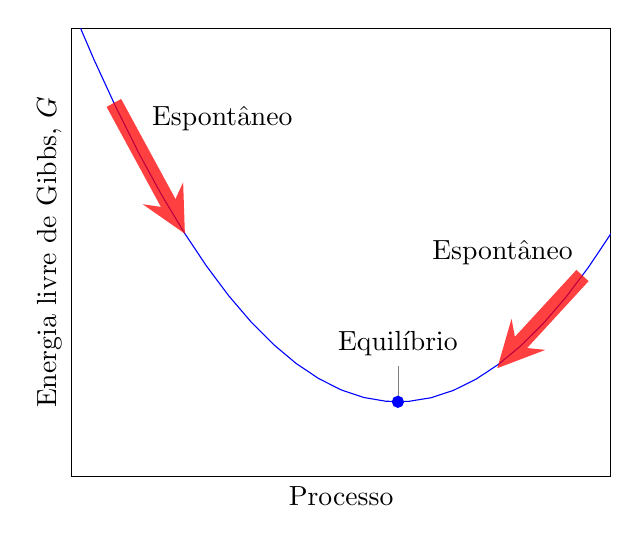
\begin{tikzpicture}
    \begin{axis}
        [
            grid = major,
            xlabel = {Processo},
            ylabel = {Energia livre de Gibbs, $G$},
            ytick = \empty,  
            xtick = \empty,
            xmin = -0.3, xmax = 3.5,
            ymin = -1, ymax = 5,
            domain = -0.3:3.5,
        ]
    \addplot [blue]
        { (x-2)^2 };

    \addplot [ mark=*, color=blue, only marks ] coordinates
        { (2, 0) };

    \begin{scope}[transparency group, opacity=0.75]
        \draw[-stealth, red, line width=0.6em] 
            (0,4) -- (0.5,2.25);
        \draw[-stealth, red, line width=0.6em] 
            (3.3,1.69) -- (2.7,0.45);
    \end{scope}
    
    \node [anchor = south west] at (axis cs:0.2,3.5) 
        { Espontâneo };

    \node [anchor = south east] at (axis cs:3.3,1.7) 
        { Espontâneo };

    \node[coordinate, pin={[fill=white] above:{Equilíbrio}}] 
        at (axis cs:2,0)   {};

    \end{axis}
\end{tikzpicture}